\subsection{How to convert a resource lead}

Thanks to our excellent opening strategy, we often found ourselves with a resource lead, even against higher rated teams. However, our bot was fantastic at throwing leads. We would quickly get out-expanded in the mid-game, and we would float\footnote{terminology from RTS games meaning to be in possesion of unused resources. You always want to fully utilize your resource, so floating resources is bad.} tons of paint in all stages of the game.

\subsection{Floating Resources}

One of the unforseen issues with only using money towers is that if they get stuck with less than 100 paint, they can never build units. This became a major issue when our soldiers would all refill on paint and leave every money tower with around 70 paint. Even with only 10 towers, this would result in us floating 700 paint. Since we were basically the only top team completely reliant on money towers, we could have a paint lead on paper, but if all of that paint was unspendable, it wasn't a paint lead in practice.

\begin{center}
    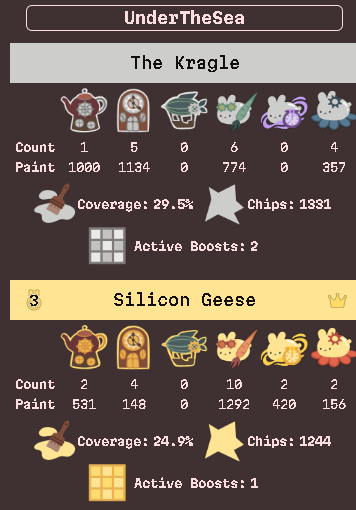
\includegraphics[scale=0.1]{images/floating_resources.png}
    \caption{We have a sizeable resource lead against Silicon Geese. However, we are floating thousands of paint in towers that could go towards making robots.}
\end{center}

\medskip

The solution was quite simple: make refilling soldiers leave precise amounts of paint required to build robots. Obviously this was a trivial fix, but the resource efficiency theory behind it was the important part.

\subsection{Reducing Idle-Time}

Besides floating resources, the other main culprit for our bot throwing leads was idle time. Often, we'd find ourselves with not just a resource lead, but a robot count lead. On paper, the team with more robots is always at an advantage. However, a robot-count lead means nothing if half of your robots are derping around.

\begin{center}
    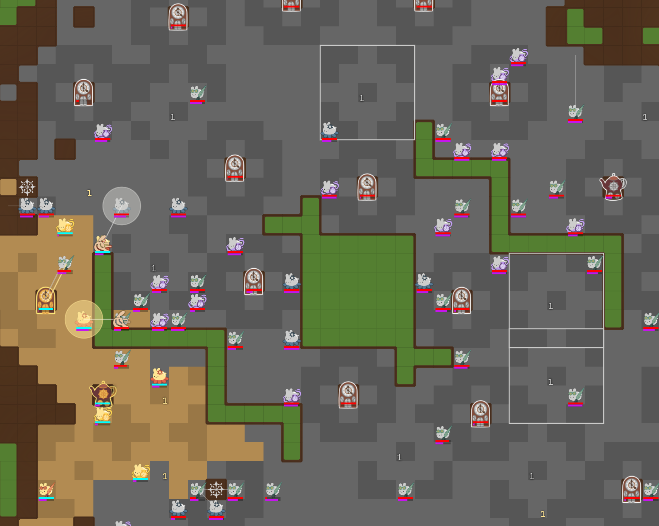
\includegraphics[scale=0.1]{images/idle_time.png}
    \caption{A gaggle of soldiers and splashers in the upper right derping around far away from where they could be useful...}
\end{center}

\medskip

The easiest idea our team had for reducing idle time was communicating battlefronts. Most games that made it to the mid/late game would result in a battlefront where both team's robots would clash near the center of the map. Without communication, our robots would explore around the map, wasting precious time, until they stumbled across a battlefront. With communication, our robots would always have knowledge of the nearest battlefront, so they could waste as little time as possible not contributing to the main fight.

\medskip

Even though our battlefront communication was mostly patchwork, it still gave massive improvements to our bot. The bots having even a vague idea about where the battlefront was reduced their idle explore time massively.

\medskip

Finally we came to the obvious realization that other teams didn't bother having their robots refill on paint. Our robots would spend about half of their lifetime travelling back to towers and waiting around towers for paint. This meant that our robots would spend about half of their lifetime in an idle state, not contributing anything.

\begin{center}
    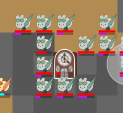
\includegraphics[scale=0.1]{images/waiting_for_refill.png}
    \caption{10 soldiers waiting for a refill on a money tower that is out of paint...}
\end{center}

\medskip

Only after we started looking carefully at what other teams were doing did we notice that no other team bothered having their bots refill on paint. This was such an obvious improvement: It cuts down on robot idle time, and allows robots to perform longer tasks at the cost of chips. You would only really want to preserve high-value robots, which was just the splashers.

\medskip

This change came way to late in the competition and was a stark reminder to pay careful attention to other team's strategies. Other teams beat your bot for a reason, and the easiest way to get your bot on the same level is to copy what they do better than you.

\subsection{Qualifiers Performance}

The bracket for Sprint 2 can be found \href{https://challonge.com/bc25javausquals}{here}.

\medskip

Thanks to our bots ability to consistently obtain a lead out of the opening and our improved efficiency, we were the 10th ranked US University team. Considering 12 US University teams make the final tournament, we were excited about our prospects of making the final tournament. However, we knew that every US University team ranked between 9th and 16th were extremely close in strength, and were likely separated more by auto-scrim luck than strength.

\medskip

The US qualifier tournament is a traditional double-elimination tournament. This means 8 teams qualify for the tournament by winning in their top 16-winners matchup, and 4 teams qualify for the tournament by wining their top 24-losers matchup. The way the team strengths were distributed, basically only the top 16 teams had a chance of qualifying. This meant that there were 4 ``quadrants'' of 4 teams, where 3 teams would make the finals. Our quadrant looked good since it included the 2 seed, the 7 seed, the 10 seed (us), and the 15 seed. If everything went according to seeding, we would lose our matchup against the 7 seed, then win our matchup against the 15 seed to qualify for the finals.

\medskip

However, disaster struck when the 15 seed, ``Podemice,'' miraculously upset the 2 seed, ``JDK? More like IDK.'' We narrowly lost our matchup against the 7 seed, ``placeholder name 2,'' in a score of 3-2. We were then given the daunting task of beating the 2 seed, ``JDK, More like IDK'' in losers. Tragically, we lost again 3-2 to be the only top 12 team not to make the finals.

\medskip

There were a few factors that made this result particularly bitter. The first was the knowledge that both of our decisive sets were 1 game away from flipping. The second was that Teh Devs didn't even do us the justice of streaming any sets from our miraculous downfall. The third and final factor was that we believed our team was top-12 strength. It just so happened that ``Podemice'' was horrifically underseeded, since they were very clearly also top-12 strength. As a result, our ``quadrant'' of the bracket was far and away the hardest one.

\medskip

The traditional bracket is designed such that the higher seeds will always have the better matchups \textbf{if no upsets occur}. This is passable in a single-elimination bracket (such as March Madness), since a lower-seed inheriting the bracket positioning of a higher-seed doesn't inherently screw anyone over. However, in a double-elimination bracket, upsets mean that a higher-seed inherits the bracket positioning of a lower-seed, which can easily screw teams over.

\medskip

Our proposed solution to this issue is bracket reseeding. This means that instead of a rigid bracket, the higher seeds will always have the better matchups regardless of whether upsets occur. As a result, instead of the 2 seed and the 10 seed battling it out for losers top 12, the 2 seed would get reseeded to play the lowest available seed (which would've been the 17 seed). This better ensures the true top-12 strength teams qualify.

\medskip

At the end of the day, we could give all the bracket-luck excuses in the world. However, that wouldn't change the fact that we couldn't win the sets that mattered most. ``Podemice,'' ``JDK? More like IDK,'' and ``placeholder name 2'' all deserved to make the finals over us, and we have nothing but the highest respect for them. In the words of Ichiro Suzuki, "I like imperfection. Because one is imperfect, it makes you want to keep moving forward."